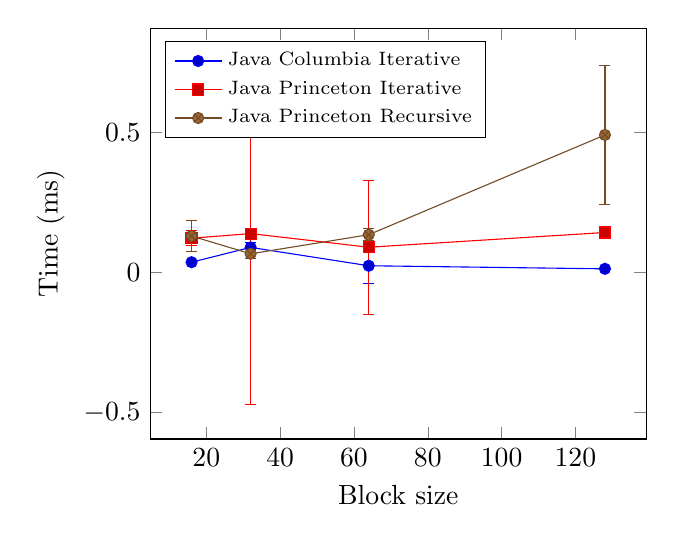
\begin{tikzpicture}
\begin{axis}[xlabel={Block size},ylabel={Time (ms)},width=0.65\linewidth,legend pos=north west,scaled y ticks = false,legend cell align=left,legend style={font=\scriptsize}]
\addplot+[error bars/.cd, y dir=both,y explicit] coordinates {
(16, 0.0370) +- (0.0055, 0.0055)
(32, 0.0899) +- (0.0169, 0.0169)
(64, 0.0244) +- (0.0637, 0.0637)
(128, 0.0134) +- (0.0005, 0.0005)
};
\addplot+[error bars/.cd, y dir=both,y explicit] coordinates {
(16, 0.1227) +- (0.0268, 0.0268)
(32, 0.1392) +- (0.6110, 0.6110)
(64, 0.0905) +- (0.2393, 0.2393)
(128, 0.1431) +- (0.0097, 0.0097)
};
\addplot+[error bars/.cd, y dir=both,y explicit] coordinates {
(16, 0.1304) +- (0.0546, 0.0546)
(32, 0.0670) +- (0.0177, 0.0177)
(64, 0.1352) +- (0.0215, 0.0215)
(128, 0.4913) +- (0.2475, 0.2475)
};
\legend{Java Columbia Iterative , Java Princeton Iterative , Java Princeton Recursive}
\end{axis}
\end{tikzpicture}
